%!TEX root = main.tex
%=================TD functions==================
\def\boldcommandlist{\@elt OP,\@elt OPs,}
\def\@elt#1,{%
 \expandafter\def\csname#1\endcsname{\textbf{#1}\xspace}
}
\boldcommandlist

\def\topColorList{\@elt TOP,\@elt TOPs,}
\def\@elt#1,{%
 \expandafter\def\csname#1\endcsname{\textcolor{TOP}{\textbf{#1}}\xspace}
}
\topColorList

\def\chopColorList{\@elt CHOP,\@elt CHOPs,}
\def\@elt#1,{%
 \expandafter\def\csname#1\endcsname{\textcolor{CHOP}{\textbf{#1}}\xspace}
}
\chopColorList

\def\sopColorList{\@elt SOP,\@elt SOPs,}
\def\@elt#1,{%
 \expandafter\def\csname#1\endcsname{\textcolor{SOP}{\textbf{#1}}\xspace}
}
\sopColorList

\def\datColorList{\@elt DAT,\@elt DATs,}
\def\@elt#1,{%
 \expandafter\def\csname#1\endcsname{\textcolor{DAT}{\textbf{#1}}\xspace}
}
\datColorList

\def\matColorList{\@elt MAT,\@elt MATs,}
\def\@elt#1,{%
 \expandafter\def\csname#1\endcsname{\textcolor{MAT}{\textbf{#1}}\xspace}
}
\matColorList


\def\compColorList{\@elt COMP,\@elt COMPs,}
\def\@elt#1,{%
 \expandafter\def\csname#1\endcsname{\textcolor{COMP}{\textbf{#1}}\xspace}
}
\compColorList

\def\redcommandlist{\@elt missingImage,\@elt testThis,}
\def\@elt#1,{%
 \expandafter\def\csname#1\endcsname{\textcolor{red}{\textbf{#1}}\xspace}
}
\redcommandlist

%===============================================

\chapter{Lecture 2, 3D Rendering}
\label{chap:3D_intro}

\section{Notes}
TOPs:\\
\begin{itemize}
  \item feedback + scale
  \item simple reaction-diffusion
\end{itemize}
Panel COMP -> Make TOP network interactive

3d Render Setup

Classic torus + noise

Panes: 3d viewport

feedback+CircleSOP+noise SOP+Panel interaction

CHOP to SOP (oscilloscope/Spectroscope)




converting between OPs\\
render setup\\
SOPs:\\
\begin{itemize}
  \item Torus
  \item Grid
  \item Sphere
  \item Noise
  \item facet
  \item transform
\end{itemize}




\begin{center}
\begin{figure}[h!]
\tikzset{concept/.append style={fill={none}}}
\begin{tikzpicture}
  \path[mindmap,concept color=textStd,text=textStd]
    node[concept] {3D}
    [clockwise from=0]
    child[concept color=TOP] {
      node[concept] (dats) {TOPs}
      [clockwise from=80]child[concept]{node[concept] {Feedback}}
    }
    child[concept color=TOP] { node[concept] {Render Setup}
        [clockwise from=270] child[concept color=MAT] { node[concept] {MATs}}
    }
    child[concept color=SOP] {
      node[concept] {SOPs}
      [clockwise from=90]
    }
    % child[concept color=CHOP] {
    %   node[concept] (dats) {Audio Analysis}
    %   [clockwise from=-30]
    % }
    child[concept color=COMP] { node[concept] (pm){COMPs}
        [clockwise from=200] child[concept]{node[concept] {Geo COMP}}
        child[concept]{node[concept] {Camera COMP}}
        child[concept]{node[concept] {Light COMP}}
        }
    child[concept color=blue] { node[concept] {GUI}
        [clockwise from=90] child[concept]{node[concept] {Panes}}
        child[concept]{node[concept] {3D Viewport}}
    };


\end{tikzpicture}
\caption{Lecture Contents}
\end{figure}
\end{center}


\newpage
\section{More TOPs}

\subsection{Feedback Networks}

\subsubsection{Reaction-diffusion}
\link{http://www.karlsims.com/rd.html}{Karl Sims Tutorial}

\begin{figure}[H]
  \centering
  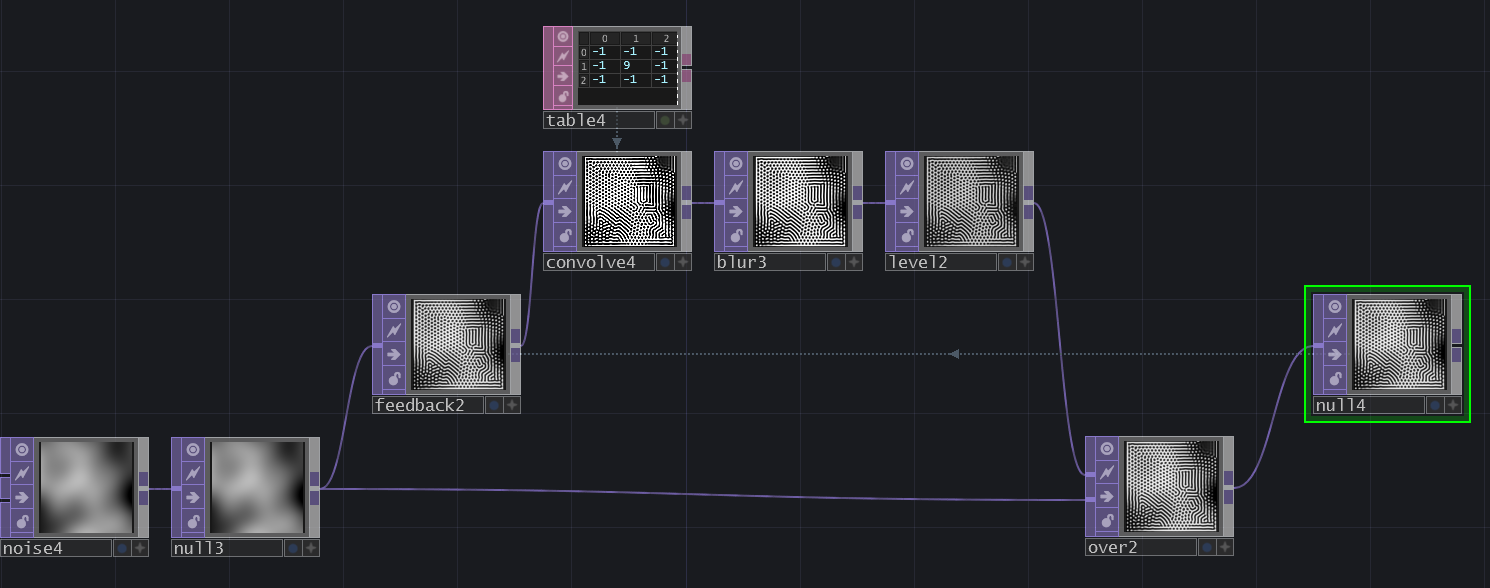
\includegraphics[width=\textwidth]{img/reactDiffuse.PNG}
  \caption[shortCaption]
  {CAPTION MISSING}
  \label{fig:label}
\end{figure}


\section{Basic Render Setup}
\index{Render Setup}
For a minimal 3D render setup we need 4 things:
\begin{itemize}
	\item Geometry \COMP
	\item Camera \COMP
	\item Light \COMP
	\item Render \TOP
\end{itemize}

\begin{figure}[H]
  \centering
  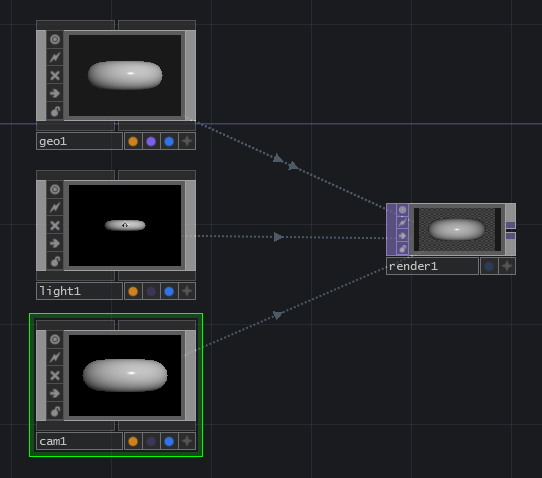
\includegraphics[width=10cm]{img/rendreSetup.PNG}
  \caption[render setup]
  {A very basic 3D rendering setup}
  \label{fig:label}
\end{figure}

\subsection{SOP Flags}


\subsection{MATs}




\subsection{Basic SOP manipulation}

\begin{figure}[H]
  \centering
  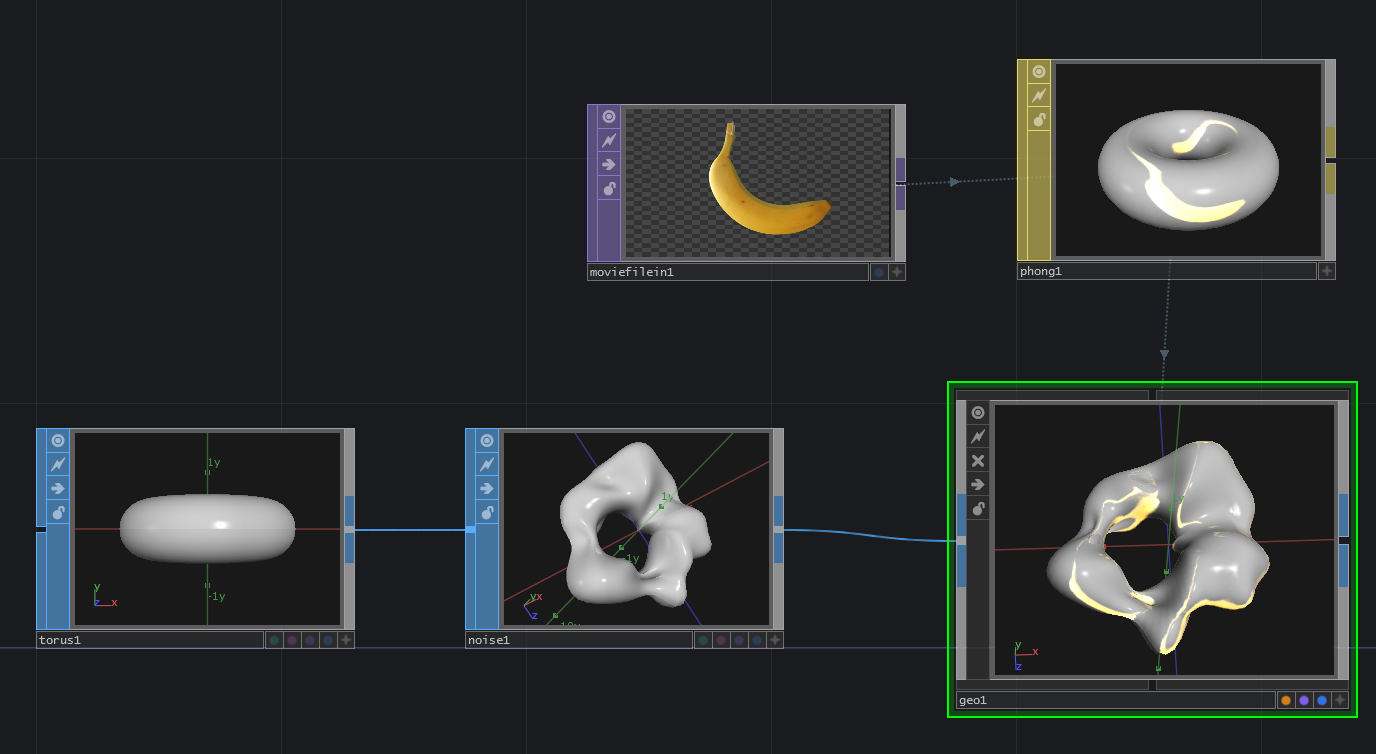
\includegraphics[width=\textwidth]{img/noise3D.PNG}
  \caption[shortCaption]
  {CAPTION MISSING}
  \label{fig:label}
\end{figure}


\subsection{The data inside a SOP}
\begin{figure}[H]
  \centering
  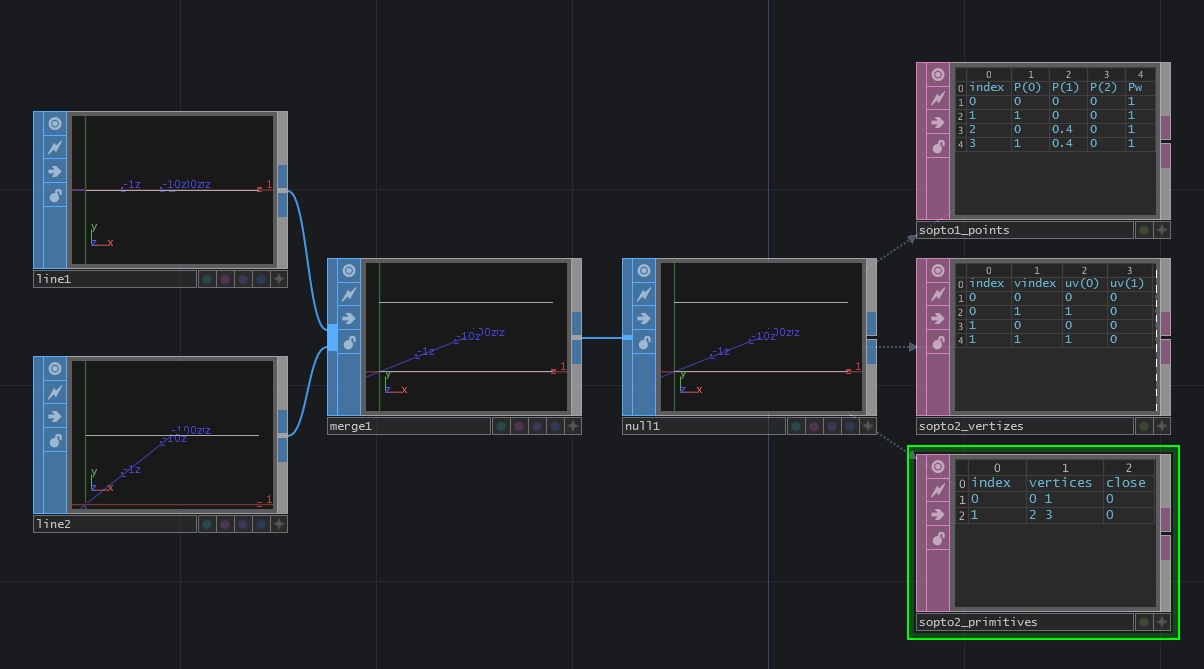
\includegraphics[width=\textwidth]{img/sopToDat.PNG}
  \caption[shortCaption]
  {CAPTION MISSING}
  \label{fig:label}
\end{figure}


\begin{framed}
  What's the difference between a point and a vertex? To quote the \link{http://derivative.ca/wiki099/index.php?title=Point}{TouchDesigner wiki}:\\
  Each SOP has a list of Points. Each point has
  \begin{itemize}
     \item an XYZ 3D position value
     \item Other optional standard attributes like RGB color, alpha, texture UV and W, Normal XYZ.
     \item user-defined attributes.
   \end{itemize}
Each polygon is defined by a vertex list, which is a list of point numbers.

So a point describes a position in 3D. A vertex is a building block of geometry that references a point. One point can be referenced by multiple vertizes.

\end{framed}